\documentclass[12pt]{book} 

\usepackage{cite}
\usepackage{graphicx}
\usepackage{geometry}
\usepackage{indentfirst} % indent first line
\usepackage{amsmath,amsthm,amsfonts,amssymb} % ams
\usepackage[normalem]{ulem} % underline emphasize
\usepackage{bm} % bold math
\usepackage{multirow} % multi row in table
\usepackage{color} % colored link
\usepackage[lastexercise]{exercise}    % exercise
\usepackage{makeidx} % index
\usepackage[linewidth=1pt,nobreak=true,framemethod=TikZ]{mdframed} % box around a content
\usepackage[titletoc]{appendix} % appendix
\usepackage{enumitem} % enumerate
\usepackage{simplewick} % wick diagram
\usepackage{tikz-cd}  % commutive diagram
\usepackage{diagbox} % slash in table
\usepackage[colorlinks]{hyperref} % color the hyperref
\usepackage{xeCJK} % Chinese support

\allowdisplaybreaks[4]  % allow to break equations 
\geometry{left=1.5cm,right=2.0cm,top=2.8cm,bottom=2.8cm}



\renewcommand{\ULdepth}{3pt}  %set uline depth
\newtheorem{theorem}{Theorem}[section]  %set theorem counter
\newtheorem{lemma}[theorem]{Lemma}  %set lemma counter
\newtheorem{axiom}[theorem]{Axiom}  %set axiom counter
\newtheorem{example}[theorem]{Example}  %set example counter
\newtheorem{method}[theorem]{Method}  %set method counter
\newtheorem{definition}[theorem]{Definition}  %set lemma counter
\newtheorem{corollary}[theorem]{Corollary}  %set lemma counter
\numberwithin{Exercise}{section}  %set exercise counter
\renewcommand\arraystretch{1.2}  % set table height

%%% in pack lastexercise
\renewcommand{\ExerciseHeader}{\leftline{\textbf{\ExerciseName\ \ExerciseHeaderNB\ExerciseHeaderTitle\ExerciseHeaderOrigin\medskip}}} %set exercise title
\renewcommand{\AnswerHeader}{\medskip\leftline{\textbf{Answer of \ExerciseName\ \ExerciseHeaderNB}\smallskip}}  %set answer title
\setlength{\ExerciseSkipBefore}{0\baselineskip}  % set spacing
\setlength{\ExerciseSkipAfter}{0\baselineskip}
\setlength{\AnswerSkipBefore}{0\baselineskip}
\setlength{\AnswerSkipAfter}{0\baselineskip}
\newenvironment{myExercise}{  %boxed exercise
	\begin{mdframed}
	\begin{Exercise}
	}{
	\end{Exercise}
	\end{mdframed}	
	}
\newenvironment{myAnswer}{  %boxed answer
		\begin{mdframed}
			\begin{Answer}
			}{
		\end{Answer}
	\end{mdframed}	
}
\newenvironment{myTabuler}{  %tabular with space
	\vspace{2ex}
	\begin{tabular}
		}{
	\end{tabular}
	\vspace{2ex}
}


\usepackage{adjustbox}
\usepackage{tikz}
\usetikzlibrary{quantikz}
\DeclareMathOperator{\tr}{tr}
\DeclareMathOperator{\diag}{diag}
\DeclareMathOperator{\Inv}{Inv}
\DeclareMathOperator{\modd}{mod}

\title{Quantum Information and Quantum Computation} 
\author{Wang Chao}
\makeindex
\begin{document} 

\maketitle 
\tableofcontents

\chapter{Foundation}

The whole universe is a large quantum system. Theoretically, any two particles in the universe are correlated. However, we usually care about physical properties of a small part of the universe. We call this part system and the rest environment. Let $|\Psi\rangle$ be a state of the universe. We can construct the state of the system as the reduced density matrix:
\begin{equation}
	\rho=\tr_{env}(|\Psi\rangle\langle\Psi|)
\end{equation}

This seems superfluous at first sight. However, in practice we lack the exact information of $|\Psi\rangle$. $\rho$ still provides the enough information we need about the system.
\section{Density Matrix}

Let $H$ be the Hilbert space of a system. From previous discussion we know that if the system is entangled with the environment, the state of the system may be described by a matrix $\rho\in H^2$. However, $\rho$ needs to satisfy a few conditions to make sense:
\begin{enumerate}
	\item $\tr\rho=1$.
	\item $\rho=\rho^\dagger$.
	\item $\rho$ is semi-positive definite.
\end{enumerate}

It's easy to see that density matrices form a convex set in $H\otimes H$, and the interior of this set contains positive definite density matrices.
\begin{definition}
	We call $\rho$ a pure state if there exists some $|\Psi\rangle\in H$ such that $\rho=|\Psi\rangle\langle\Psi|$. Otherwise we call $\rho$ a mixed state.
\end{definition}

\begin{lemma}
	Only pure states are extremal points(points that are not linear combination of other points).
\end{lemma}
\begin{proof}
	Since $\rho$ is semi-positive definite, $\langle a|\rho|a\rangle=0\rightarrow\rho|a\rangle=0$. Let $\rho=|\Psi\rangle\langle\Psi|$ be a pure state. If $\rho=\lambda\rho_1+(1-\lambda)\rho_2$ and $\lambda\neq0,1$. Then for each $|\Psi^\perp\rangle$ perpendicular to $|\Psi\rangle$, $\langle \Psi^\perp|\rho_1|\Psi^\perp\rangle=\langle \Psi^\perp|\rho_2|\Psi^\perp\rangle$=0. This leads to that $\rho_1=\rho_2=|\Psi\rangle\langle\Psi|$.
\end{proof}

\section{Orthogonal Measurement}

Let $O=O_{sys}\otimes I_{env}$ be an observable in the universe. We can decompose $O_{sys}=\sum_i o_iP_i$, where
\begin{enumerate}
	\item $P_i$ is Hermitian
	\item $\sum_i P_i=I$
	\item $P_iP_j=\delta_{ij}P_i$
\end{enumerate}
$P_i$ is the projective operator into the subspace with eigenvalue $o_i$. The measurement can also be denoted by $(o_i,P_i)$. After measurement, the state $|\Psi\rangle$ has the chance $\parallel P_i\otimes I|\Psi\rangle\parallel^2$ to collapse into the state $P_i\otimes I|\Psi\rangle/\parallel P_i\otimes I|\Psi\rangle\parallel$, with measure value $o_i$.

If we represent the state of the system by density matrix $\rho=\tr_{env}(|\Psi\rangle\langle\Psi|)$. Then the state has the chance
\begin{equation}
	\parallel P_i\otimes I|\Psi\rangle\parallel^2=\langle \Psi|( P_i\otimes I)^2|\Psi\rangle=\tr(P_i^2\otimes I|\Psi\rangle\langle\Psi|)=\tr_{sys}(P_i^2\rho)
\end{equation}
to collapse into the state
\begin{equation}
	\tr_{env}(P_i\otimes I|\Psi\rangle\langle\Psi|P_i\otimes I)/\tr_{sys}(P_i^2\rho )=P_i\rho P_i/\tr_{sys}(P_i^2\rho)
\end{equation}
with measure value $o_i$.

\section{Positive Operator-valued Measure}

Let's consider a more general measure $(o_i,E_i)$, where
\begin{enumerate}
	\item $E_i$ is Hermitian
	\item $\sum_i E_i=I$
	\item $E_i$ is semi-positive
\end{enumerate}

After measurement, the state $\rho$ has the chance $tr(E_i\rho)$ to collapse into the state $M_i\rho M_i^\dagger/\tr(E_i\rho)$ where $E_i=M_i^\dagger M_i$.

This is called positive operator-valued measure(POVM).

POVM can be realized by entangle the system with an auxiliary space $\rho\rightarrow \rho\otimes|0\rangle\langle 0|\in (H_{sys}\otimes H_{aux})^2$. We find a unitary transformation $U$ such that $U|\psi\rangle\otimes|0\rangle=\sum_i (M_i|\psi\rangle)\otimes |i\rangle$. The existence of $U$ is equivalent to that $\sum_i M_i^\dagger M_i=I$. Then POVM can be realized by measuring $H_{sys}\otimes H_{aux}$ by $(o_i,I\otimes |i\rangle\langle i|)$. 

\section{Quantum Channel}

A quantum channel is a linear map of density operator
\begin{equation}
	\mathcal E(\rho)=\sum_aM_a\rho M_a^\dagger
\end{equation}
where $\{M_a\}$ be a set of operators such that $\sum_a M_a^\dagger M_a=I$, called Kraus operators of the channel. 

A quantum channel has following easily verified properties:
\begin{definition}
	A trace-preserving completely positive map $\mathcal E$ is a linear map that
	\begin{enumerate}
		\item Preserves positivity completely, that is, $I_k\otimes\mathcal E$ preserves Hermiticity and positivity for all positive integer $k$: $\rho=\rho^\dagger\rightarrow I_k\otimes \mathcal E(\rho)= I_k\otimes \mathcal E(\rho)^\dagger$ and $\rho\geq 0\rightarrow I_k\otimes\mathcal E(\rho)\geq 0$
		\item Preserves trace: $\tr(\mathcal E(\rho))=\tr(\rho)$	
	\end{enumerate}
\end{definition}
\begin{lemma}
	A quantum channel is a trace-preserving completely positive map
\end{lemma}
\begin{lemma}
	A trace-preserving completely positive map is a quantum channel
\end{lemma}
\begin{proof}
	Let $\mathcal E(\rho)_{kl}=\rho_{ij}C_{ijkl}$. Since $C_{ijkl}$ is completely positive, by Choi's theorem, $C_{ijkl}=C^*_{jilk}$ and $C_{ijkl}$ is semi-positive between $ik$ and $jl$. The former is obvious and the latter can be seen from the positivity of $I_n\otimes \mathcal E$, as illustrated in Fig. \ref{fig:complete_positive}. Thus $C_{ijkl}=\sum_a M_{aki}M^*_{alj}$. Since $C_{ijkl}$ preserves trace, $\sum_a M_a^\dagger M_a=I$.
\end{proof}

\begin{figure}[htb!]
	\centering  
	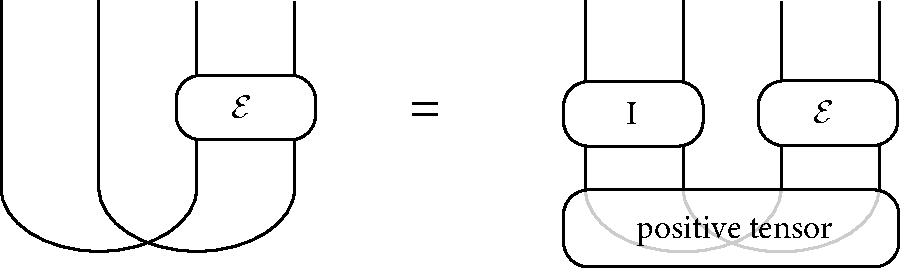
\includegraphics[scale=0.6 ]{fig/complete_positive.pdf}  
	\caption{Positivity of trace-preserving completely positive map}
	\label{fig:complete_positive}
\end{figure}

\begin{definition}
	A quantum channel $\mathcal E$ is called unitary if $\mathcal E(\rho)=U\rho U^\dagger$ for a unitary operator $U$.
\end{definition}

\begin{lemma}
	Let $A_{ijkl}$ and $B_{ijkl}$ be two tensors of index dimension $N$, such that
	\begin{enumerate}
		\item $A_{ijkl}=A^*_{klij}$ and $A_{ijkl}$ is semi-positive between $ij$ and $kl$
		\item $B_{ijkl}=B^*_{klij}$ and $B_{ijkl}$ is semi-positive between $ij$ and $kl$
		\item $A_{ijkl}B_{jmln}=\delta_{im}\delta_{kn}$
	\end{enumerate}
	Then $A_{ijkl}=a^*_{ij}a_{kl}$ and $B_{ijkl}=b^*_{ij}b_{kl}$.
	
	The lemma can be expressed in graphical language. Let \adjustbox{valign=c}{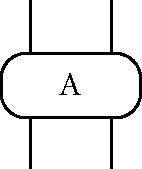
\includegraphics[scale=0.5]{fig/tensor_A.pdf}} and \adjustbox{valign=c}{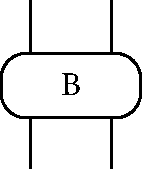
\includegraphics[scale=0.5]{fig/tensor_B.pdf}} be Hermitian and semi-positive tensors between their left and right indices, and \adjustbox{valign=c}{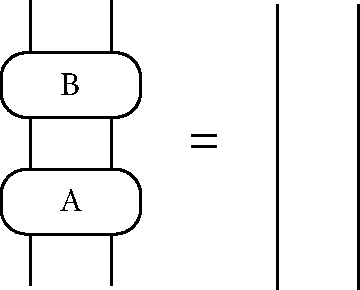
\includegraphics[scale=0.5]{fig/tensor_AB.pdf}} . Then \adjustbox{valign=c}{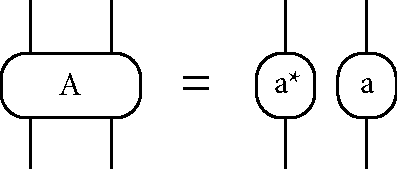
\includegraphics[scale=0.5]{fig/tensor_A_dec.pdf}} and \adjustbox{valign=c}{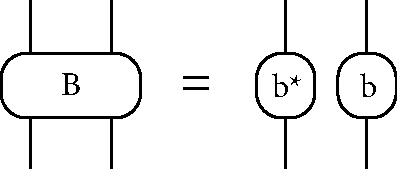
\includegraphics[scale=0.5]{fig/tensor_B_dec.pdf}} .
\end{lemma}
\begin{proof}
	Let's define $D(\alpha,\beta)$ as the Schmidt dimension between index $\alpha$ and $\beta$.
	
	Clearly \adjustbox{valign=c}{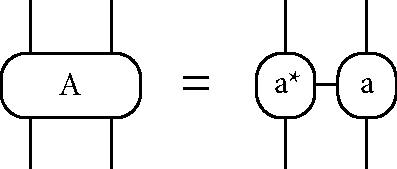
\includegraphics[scale=0.5]{fig/tensor_A_dec2.pdf}} and \adjustbox{valign=c}{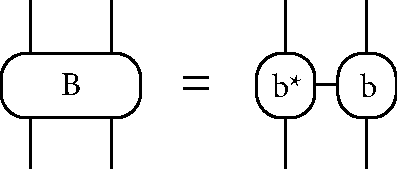
\includegraphics[scale=0.5]{fig/tensor_B_dec2.pdf}} . Since \adjustbox{valign=c}{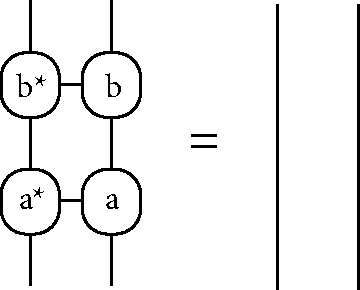
\includegraphics[scale=0.5]{fig/tensor_aabb.pdf}} , $D(ij,kl)=1$ for \adjustbox{valign=c}{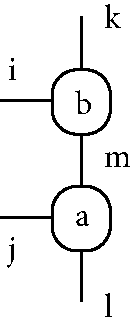
\includegraphics[scale=0.5]{fig/tensor_ab_ind.pdf}} . That means \adjustbox{valign=c}{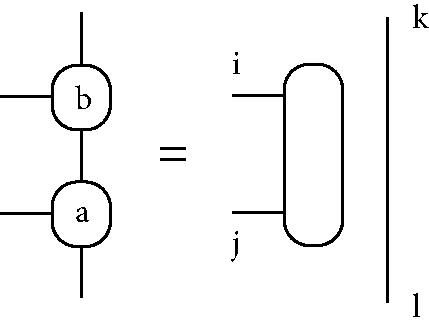
\includegraphics[scale=0.5]{fig/tensor_ab3.pdf}} . Clearly $D(i,j)\cdot D(k,l)=D(i,j)\cdot N=D(ij,kl)\leq N$ for RHS. So $D(i,j)=1$ and $D(ij,kl)= N$, which means \adjustbox{valign=c}{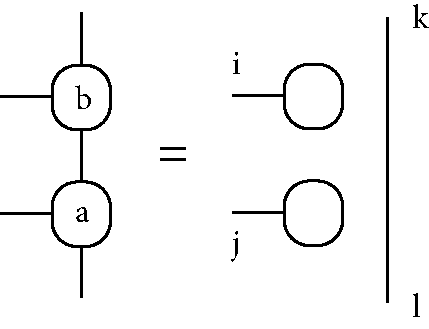
\includegraphics[scale=0.5]{fig/tensor_ab4.pdf}}. So for \adjustbox{valign=c}{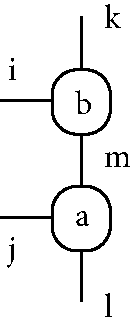
\includegraphics[scale=0.5]{fig/tensor_ab_ind.pdf}}, $D(i,jkl)=D(j,ikl)=1$ and $D(ij,kl)= N$. From this we can deduce that $D(i,km)=D(j,lm)=1$. Thus \adjustbox{valign=c}{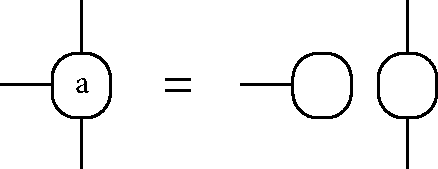
\includegraphics[scale=0.5]{fig/tensor_a_simp.pdf}} and \adjustbox{valign=c}{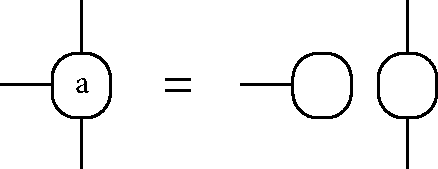
\includegraphics[scale=0.5]{fig/tensor_a_simp.pdf}} . Hence \adjustbox{valign=c}{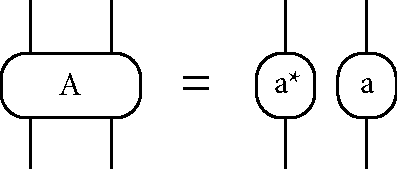
\includegraphics[scale=0.5]{fig/tensor_A_dec.pdf}} and \adjustbox{valign=c}{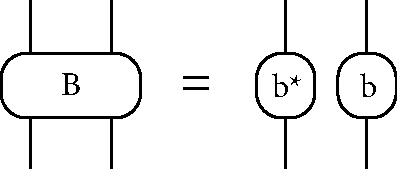
\includegraphics[scale=0.5]{fig/tensor_B_dec.pdf}} .
\end{proof}

\begin{corollary}
	A quantum channel is invertible iff it's unitary.
\end{corollary}

\section{Evolution}

The quantum channel is a model to describe the evolution of the system with entanglement to the environment. We assume that initially there's no entanglement between the system and the environment. The state of the universe is
\begin{equation}
	\rho_{univ}=\rho_{sys}\otimes \rho_{env}
\end{equation}

This may sound absurd since if there's no entanglement between the system and the environment, the system is in pure state. So we may modify our assumption. We assume that the system has no entanglement with its nearby environment. The system may have entanglement with some remote part of the environment. That is, the state of the universe of a local region around the system is
\begin{equation}
	\rho_{local}=\rho_{sys}\otimes \rho_{nb\ env}
\end{equation}

After a short period of time, the local region evolve by a unitary evolution $U$.
\begin{equation}
	\rho_{local}'=U\rho_{local}U^\dagger+\rho_{int}
\end{equation}
where $\rho_{ent}$ described the impact of the interaction between the local region and the rest.

The system would be in state
\begin{equation}
	\rho_{sys}'=\tr_{nb\ env}[U\rho_{local}U^\dagger]+\tr_{nb\ env}\rho_{int}
\end{equation}

Here we may omit the influence of interaction between the local region and the rest on the state of the system, since it only has local impact. Then
\begin{equation}
	\rho_{sys}'=\tr_{nb\ env}[U\rho_{sys}\otimes \rho_{nb\ env}U^\dagger]
\end{equation}


This is a quantum channel with transformation tensor $C_{ijkl}=\delta_{ik}\delta_{jl}+\mathcal O(dt)$. Let
\begin{equation}
	C_{ijkl}=\sum_a \lambda_aU_{a,ki}U^*_{a,lj}
\end{equation}

Since $C_{ijkl}C_{jilk}=\sum_i\lambda_i^2=D^2+\mathcal O(dt)$ and $C_{ijij}=\sum_i\lambda_i=D+\mathcal O(dt)$. We have $\lambda_0=D+\mathcal O(dt)$ and $\lambda_i=\mathcal O(dt)$ when $i>0$.
 
Then
\begin{equation}
	\lambda_0U_{0,ki}U^*_{0,lj}=\delta_{ik}\delta_{jl}+\mathcal O(dt)
\end{equation}
By contraction with $\delta_{ik}$ on both sides, we see that $U_{0,ij}=e^{i\theta}\frac 1{\sqrt D}\delta_{ij}+\mathcal O(dt)$.

Then we conclude
\begin{equation}
	C_{ijkl}=\sum_a M_{aki}M^*_{alj}
\end{equation}
where
\begin{align}
	M_{0ij}&=\delta_{ij}-idtH_{ij}+dtK_{ij}\\
	M_{aij}&=\sqrt{dt} L_{aij}\quad(a>0)
\end{align}
Here, $H$ and $K$ are Hermitian. $H$, $K$ and $L_a$ are $\mathcal O(1)$. 

Since  $\sum_a M_a^\dagger M_a=I$, we have $2K=-\sum_{a>0}L_a^\dagger L_a$.

Let $\mathcal E$ and $\mathcal E'$ be two infinitesimal quantum channels with Hamiltonian $H$ and $H'$ and Lindblad operators $\{L_a\}$ and $\{L'_a\}$. Then $\mathcal E\circ\mathcal E'=\mathcal E'\circ \mathcal E$ is the quantum channels with Hamiltonian $H+H'$ and Lindblad operators $\{L_a,L'_a\}$.

\section{Markovian Evolution}

Let's consider an evolution process from $t_0$ to $t_2$. As before, we assume the state at $t_0$ has no entanglement with its nearby environment. However, at each $t_1\in (t_0,t_2)$, the system has entanglement with its nearby environment. So the quantum channel from $t_0$ to $t_2$ is not the composition of one from $t_0$ to $t_1$ and one from $t_1$ to $t_2$. In other words, the evolution from $t_1$ to $t_2$ requires information of the environment that has been transferred from the system during the time period from $t_0$ to $t_1$. The evolution is non-Markovian.

However, if we make the assumption has the the information transferred from the system to the environment dissipate really fast. Then at each time, the system has no entanglement with its nearby environment. Then the global quantum channel is the composition of infinitesimal quantum channels:
\begin{equation}
	\mathcal E_{t\rightarrow t'}=\mathcal E_{t'-\Delta t\rightarrow t'}\circ\cdots\circ\mathcal E_{t\rightarrow t+\Delta t}
\end{equation}

The evolution of the system can be described by a differential equation
\begin{align}
	\rho(t+\Delta t)&=\sum_a M_a\rho(t) M_a^\dagger\\
	&=(I-idtH+dtK)\rho(t)(I+idtH+dtK)+\sum_{a>0}L_a\rho L_a^\dagger\\
	\dot \rho&=-i[H,\rho]+\sum_{a>0}(L_a\rho L_a^\dagger-\frac 12\rho L_a^\dagger L_a-\frac 12L_a^\dagger L_a\rho )
\end{align}

\chapter{Entanglement}

\chapter{Quantum Information}

\chapter{Quantum Computation}

\section{Quantum Fourier Transformation on $\mathbb Z_{2^n}$}

The Fourier transformation is the unitary operator $F_N$ such that
\begin{equation}
	F_N\sum_x f(x)|x\rangle=\frac 1{\sqrt{N}}\sum_y\sum_x f(x)e^{2\pi ixy/N}|y\rangle
\end{equation}

For each basis vector $|x\rangle$,
\begin{equation}
	F_N|x\rangle=\frac 1{\sqrt{N}}\sum_y e^{2\pi ixy/N}|y\rangle
\end{equation}

Let $N=2^n$, and
\begin{align}
	x&=\sum_i x_i2^i\\
	y&=\sum_i y_i2^i
\end{align}

Then
\begin{equation}
	xy=\sum_i y_i2^i\sum_j x_j2^j\equiv \sum_i y_i\sum_{i+j<n} x_j2^{i+j} \mod N
\end{equation}

The Fourier transformation on a basis becomes
\begin{align}
	F_N|x\rangle &=\frac 1{\sqrt{N}}\sum_y e^{2\pi i\sum_i y_i\sum_{i+j<n} x_j2^{i+j} /N}|y\rangle\\
	&=\frac 1{\sqrt{N}}\bigotimes_{i=0}^{n-1}\sum_{y_i}e^{2\pi i y_i\sum_{i+j<n} x_j2^{i+j} /N}|y_i\rangle\\
	&=\bigotimes_{i=0}^{n-1}\frac 1{\sqrt{2}}(|0\rangle+e^{2\pi i\sum_{i+j<n} x_j2^{i+j-n}}|1\rangle)\\
	&=\Inv\bigotimes_{i=0}^{n-1}\frac 1{\sqrt{2}}(|0\rangle+e^{\pi i\sum_{j\leq i} x_j2^{j-i}}|1\rangle)\\
	&=\Inv\prod_{i=n-1}^{0} \prod_{j=i-1}^0R_{ji}(i-j)H_i|x\rangle
\end{align}
where $H_i$ is Hadamard gate on qubit $i$, $\Inv$ is the operator $|x_0\dots x_{n-1}\rangle\mapsto|x_{n-1}\dots x_0\rangle$, and $R_{ji}(d)$ is operator $\diag(1,e^{i\pi/2^d})$ on qubit $i$ controlled by qubit $j$.
\begin{center}
\begin{quantikz}
\lstick{$|x_3\rangle$} &\gate{H} &\gate{R(1)} &  \gate{R(2)} & \gate{R(3)}& \qw& \qw & \qw & \qw   & \qw& \qw&\swap{3} & \qw &\qw\\
\lstick{$|x_2\rangle$} &\qw&\ctrl{-1} &\qw & \qw &\gate{H}&\gate{R(1)}& \gate{R(2)}& \qw& \qw& \qw& \qw  &\swap{1}&\qw \\
\lstick{$|x_1\rangle$}  &\qw &\qw &  \ctrl{-2}& \qw &\qw &\ctrl{-1}& \qw& \gate{H} &\gate{R(1)}& \qw& \qw&\targX{} &\qw\\
\lstick{$|x_0\rangle$} & \qw &\qw &\qw& \ctrl{-3} & \qw& \qw & \ctrl{-2}& \qw & \ctrl{-1} &\gate{H}&\targX{}& \qw&\qw
\end{quantikz}
\end{center}

This method can be generalized into quantum Fourier transformation on a ring $\prod_i\mathbb Z_{N_i}$.

\section{Period Finding}

Let $f(x)$ be a periodic function on $\mathbb Z_N$ with period $r$. Let's suppose there's a unitary transformation $U:|x\rangle|0\rangle\mapsto |x\rangle|f(x)\rangle $. Choose $N> r^2$. Then

\begin{equation}
	U\sum_{x=1,\dots,N}|x\rangle|0\rangle=\sum_{x=1,\dots,N}|x\rangle|f(x)\rangle
\end{equation}

Then let's measure the second register and get result $a$. The state in first register becomes
\begin{equation}
	\sum_{x=1,\dots,N,f(x)=a}|x\rangle=\sum_{n=1,\dots,M}|x_0+nr\rangle
\end{equation}
where $x_0j$ is the smallest integer such that $f(x_0)=a$, and $x_0+Mr$ is the largest integer.

After quantum Fourier transformation, the state becomes
\begin{equation}
	\frac 1{\sqrt{N}}\sum_{q=1,\dots,N}(\sum_{n=1,\dots,M}e^{2\pi i(x_0+nr)q/N})|q\rangle
\end{equation}
The peaks of this distribution is at $\frac q N=\frac j r$. By Preskill, the probability of measured value of $\frac q N$ to fall in $[\frac j r-\frac 1{2N},\frac j r+\frac 1{2N}]$ for some $j$ is $>\frac 4{\pi^2}$. If we measure $\frac q N$ and approximated the result, which is close to $\frac j r$, by a rational $\frac a b$ such that $b<\sqrt N$, clearly $a/b=j/r$. Thus we can obtain $\frac j r$ by applying continued fraction algorithm to the measure value of $\frac q N$. Chances are that $j$ and $r$ are coprime, and we obtain $r$.

This method can be generalized into functions over a ring $\prod_i\mathbb Z_{N_i}$, such Simon's method on $\mathbb Z_2^{\otimes n}$.

\section{Shor Algorithm}

The algorithm to factor a number $N$ is
\begin{enumerate}
	\item Randomly choose a number $a<N$ coprime to $N$
	\item Use quantum algorithm to find smallest $r$ such that $a^r\equiv 1 \modd N$.
	\item If $r$ is odd, change $a$ and restart. If $r$ is even, we have $(a^{r/2}+1)(a^{r/2}-1)\equiv 0 \modd N$
	\item Clearly $(a^{r/2}-1)\not\equiv 0 \mod N$. If $(a^{r/2}+1)\equiv 0 \modd N$, change $a$ and restart. Otherwise, $gcd(a^{r/2}+1,N)$ is a nontrivial divisor of $N$.
\end{enumerate}

$r$ can be obtained by finding the period of the function
\begin{equation}
	f_{a,N}(x)=a^x \modd N
\end{equation}
using the previous algorithm. 

Here we provide the quantum circuit to perform $U|x\rangle|1\rangle=|x\rangle |f_{a,N}(x)\rangle$. Let's express $x$ as a binary expansion
\begin{equation}
	x=\sum_i x_i\cdot 2^i
\end{equation}

Then
\begin{equation}
	a^x \modd N=a^{\sum_i x_i\cdot 2^i}\modd N=\prod (a^{2^i})^{x_i}\modd N=\prod (a_i)^{x_i}\modd N
\end{equation}
where $a_i=(a^{2^i}) \modd N$ and can be calculated by $a_i=(a_{i-1})^2\mod N$.

The quantum circuit to perform $U|x\rangle|1\rangle=|x\rangle |f_{a,N}(x)\rangle$ is
\begin{center}
\begin{quantikz}
\lstick{$|x_2\rangle$} &[4mm]\qw & \qw & \ctrl{3} &\qw \\
\lstick{$|x_1\rangle$} &[4mm] \qw &\ctrl{2} & \qw &\qw \\
\lstick{$|x_0\rangle$}  &[4mm] \ctrl{1}\qw  & \qw & \qw &\qw \\
\lstick{$\ket{0}$} &[4mm] \gate{\times a}\qwbundle{n} & \gate{\times a^2}& \gate{\times a^4} & \qw 
\end{quantikz}
\end{center}
where $|1\rangle$ is encoded by $|0\rangle^{\otimes n}$. 

The whole circuit of Shor's algorithm is 
\begin{center}
\begin{quantikz}
\lstick{$|0\rangle$} &\gate{H} &\qw &  \qw & \ctrl{3} & \gate[wires=3][2cm]{QFT}&\qw  \\
\lstick{$|0\rangle$} &\gate{H}&\qw & \ctrl{2} & \qw &\qw &\qw  \\
\lstick{$|0\rangle$}  &\gate{H} & \ctrl{1}\qw  & \qw & \qw &\qw &\qw  \\
\lstick{$\ket{0}$} & \qw \qwbundle{n}& \gate{\times a} & \gate{\times a^2}& \gate{\times a^4} & \qw\rstick{$\ket{0}$}
\end{quantikz}
\end{center}
\chapter{Quantum Error Correction}
	
\chapter{Topological Quantum Computation}
%\appendix
% Here to insert appendix

%\printindex
%\bibliographystyle{unsrt}
%\bibliography{mybib}
\end{document}